\AuthorInfo{
name=,
headings=\textsc{Luca De Feo},
institution={IBM Research GmbH},
address={Säumerstrasse 4, Rüschlikon, Schweiz},
email={aracne-2021@defeo.lu},
} %da inserire all'inizio del contributo


\chapter[toc=Isogenies Demystified\\{\protect\small\emph{Luca De Feo}}, headings=Isogenies Demystified]{Isogenies Demystified\\\vspace{2mm}\normalsize \textsc{Luca De Feo}\protect}

\addtocontents{toc}{\protect\vspace{-4mm}}

\begin{otherlanguage}{english}
  \def\Z{\mathbb{Z}}
  \def\Q{\mathbb{Q}}
  \def\F{\mathbb{F}}
  \def\exp{\mathrm{exp}}
  \def\com{\mathcal{C}}
  \def\Gal{\mathrm{Gal}}
  \def\End{\mathrm{End}}
  \def\Ell{\mathrm{Ell}}
  \def\Cl{\mathrm{Cl}}
  \def\O{\mathcal{O}}
  
  Isogenies, what are they? Like the character in Alessandro Manzoni's
  novel, cryptographers encountering an isogeny in a textbook would
  have been justified, ten years ago, asking themselves ``\textit{chi
    era costui?}''\footnote{``Who was he?'', inquires Don Abbondio
    upon reading the name of Carneades in a hagiography of St Charles
    Borromeo.} Elliptic curves, that, we know. But isogenies?  The
  name sounds familiar, it must be one of those math things starting
  in iso-; but \textit{chi diavolo era costui?}\footnote{There would
    be much to say about how Manzoni's \textit{faux savant}
    characters, from Don Abbondio to Don Ferrante, speak of our
    time. But this is an article about isogenies.}

  That is no longer true. Any self-respecting cryptographer nowadays
  must have at least a vague idea of what isogenies are and how they
  are used in cryptography. This survey is your guide to the
  supersingular isogeny galaxy~\cite{galaxy}.

  \section{\textit{Aufstieg und Fall der Elliptische-Kurven-Kryptografie}}
  Elliptic curves are today a fact of life.  I sometimes wonder what
  Euler would have thought of it.  Not a single day goes without
  billions of elliptic curve operations being performed by servers,
  laptops, smartphones and even refrigerators throughout the world. I
  suppose Euler would have loved the fridge.

  Why are elliptic curves so important in cryptography? One reason is
  that they are the closest thing we know to a \emph{generic
    group}. What cryptographers ask from a group is: to be abelian, to
  be finite, to have efficient algorithms for testing membership,
  equality, and for evaluating the group operation. Any group well
  mannered enough to do exactly what is asked from it, and nothing
  more, is called \emph{generic}.

  The most important operation for a cryptographic group is
  \emph{exponentiation}:
  \begin{align*}
    \exp_g : \Z &\to G,\\
    x &\mapsto g^x.
  \end{align*}
  That $\exp_g(n)$ can be evaluated using $O(\log(n))$ generic group
  operations is obvious. What makes a group precious is the inverse
  map $g^x\mapsto x$, the \emph{discrete logarithm}, being
  ``difficult'' to compute. Then $\exp_g$ is what cryptographers call
  a \emph{one-way function}.

  The other reason groups are loved, and I claim it is the most
  important one, is that no knowledge of number theory is required
  in order to make cryptography out of them.  Cryptography is like
  humanity in Plato's cave: it only sees the tame generic group shadow
  of a wild real world elliptic curve. Do not get me wrong: this is
  great! We wouldn't have as powerful cryptographic tools, if creating
  them required a deep knowledge in number theory. We do not have such
  a luxury with isogenies.
  
  What can you do with a generic group? A lot of things. I am sure the
  reader is familiar with the Diffie--Hellman key
  exchange~\cite{DifHel76}, but I want to highlight a different
  application. A \emph{commitment scheme} is the cryptographic
  equivalent of a sealed envelope: in the first phase a party
  \emph{commits to} a message $m$ (\emph{e.g.}, a monetary offering)
  by publishing a \emph{commitment} $\com(m;r)$, where $r$ represents
  an arbitrary auxiliary input (typically, some random bits); in the
  second phase, the party \emph{opens} the commitment by revealing $m$
  and $r$; anyone can check that $m$ is the message originally
  committed to by recomputing $\com(m;r)$.  A cryptographic commitment
  must satisfy two properties: it must be \emph{binding}, \emph{i.e.},
  after having committed to $\com(m;r)$ it must be difficult for the
  party to find $(m',r')$ with $m\ne m'$ such that
  $\com(m';r')=\com(m;r)$; and it must by \emph{hiding}, \emph{i.e.},
  given only $\com(m;r)$ it must be difficult to deduct $m$.  A
  commitment is \emph{perfectly binding} when $\com(m;r)$ is
  injective; \emph{perfectly hiding} when the output of $\com(m;r)$ is
  uncorrelated to $m$, assuming $r$ is drawn from some probability
  distribution. It is easy to see that the two perfect properties are
  mutually exclusive.

  Given a generic group $G$ with some fixed generator $g$, it is easy
  to imagine a simple commitment scheme defined by $\com(m) =
  g^m$. This scheme is obviously binding if $0<m<\#G$, and is hiding
  thanks to the one-wayness of the $\exp_g$ function. However, while
  the binding property is \emph{perfect}, the hiding property only
  holds against \emph{computationally bounded} adversaries. This may
  be a problem if, for example, the messages $m$ are likely to be
  taken from a small subset.

  Pedersen~\cite{C:Pedersen91} is credited with a very simple and
  elegant idea to obtain a perfectly hiding commitment scheme from
  generic groups. Let $g$ and $h$ be two random generators of $G$, he
  defined $\com(m;r)=g^m h^r$, where $r$ is a random integer in
  $[1,\#G]$. It is easy to see that Pedersen's commitment is perfectly
  hiding, thanks to $h^r$ being uniformly distributed in $G$. For the
  binding property, it is capital that the discrete logarithm relation
  between $g$ and $h$ is unknown to the committer; indeed, given
  $x=\log_g(h)$ the commitment simply becomes $g^{m+xr}$, and breaking
  binding simply amounts to solving the equation $m+xr=m'+xr'$ modulo
  $\#G$.

  Pedersen commitments can do much more than just emulate digital
  envelopes, and in fact a great variety of cryptographic protocols is
  based on them and similar ideas. Most of the advanced cryptographic
  protocols used nowadays, such as the Signal protocol used by
  WhatsApp, or those used in privacy-preserving cryptocurrencies, use
  some advanced features of generic groups such as Pedersen
  commitments; and their generic group of choice is, inevitably,
  elliptic curves.

  But the reader knows the story by now: our world is coming to an
  end, Shor's bane is free~\cite{FOCS:Shor94}, soon hordes of quantum
  computers will roam the earth, mercilessly hunting down discrete
  logarithms and composite integers, our mobile data plans will
  evaporate in just days to accommodate for post-quantum cryptography.

  \section{Isogeny graphs}
  I will assume some familiarity with elliptic curves and abstract
  algebra. Just so that we are on the same page, I will fix some
  notation once and for all.

  \paragraph{Notation.} $R[x]$ denotes the algebra generated by an
  element $x$ over a ring $R$, while $k(y)$ denotes the field
  extension generated by an element $y$ over a field $k$.  When $E$ is
  an elliptic curve, these are not to be confused with $E[n]$ ---the
  subgroup of $n$-torsion points--- and with $E(k)$ ---the subgroup of
  $k$-rational points for some field $k$. When $a,b,\ldots$ are group
  elements, $\langle a,b,\ldots\rangle$ denotes the subgroup generated
  by them. Finally, when $\phi$ is a group morphism, $\ker\phi$
  denotes its kernel.

  At this point, we are obliged to choose a camp in a
  controversy as ancient as ``Emacs vs vi'': unlike cryptographers,
  algebraists like to write abelian groups additively. We will side
  with the algebraists and rewrite exponentiation as
  \[[n]P := \exp_P(n),\] with the side-effect of loosing track of
  the original meaning of ``discrete logarithm''.

  The \emph{multiplication map} $[n]$ is an example of a morphism from
  an elliptic curve to itself.  Isogenies are generalizations of these
  morphisms, when we view elliptic curves both as groups and as
  algebraic varieties.

  \begin{definition}
    Let $\varphi:E\to E'$ be a map between two elliptic curves defined
    over an algebraically closed field, the following are equivalent:
    \begin{enumerate}
    \item $\varphi$ is a surjective group morphism,
    \item $\varphi$ is a group morphism with finite kernel,
    \item $\varphi$ is a non-constant algebraic map of projective
      varieties sending the point at infinity of $E$ onto the point at
      infinity of $E'$.
    \end{enumerate}
    In any of these cases, $\varphi$ is called an \emph{isogeny}; or
    an \emph{endomorphism} when $E=E'$.
  \end{definition}

  In cryptography, however, we typically deal with non-algebraically
  closed fields. In this case, we need to take \emph{rationality} into
  account. Let $k$ be a field with algebraic closure $\bar{k}$. By
  $E/k$ we mean a curve defined over $k$, \emph{i.e.}, whose equation
  has coefficients in $k$. We can extend scalars to $\bar{k}$, and see
  $E$ as a curve over $\bar{k}$; when it is necessary to distinguish
  between them, we will write $E(\bar{k})$ for the group of points in
  the algebraic closure, and $E(k)$ for the group of
  \emph{$k$-rational} points.  Then the Galois group of $\bar{k}/k$
  acts on $E(\bar{k})$ by permuting its elements.

  \begin{definition}
    Let $E$, $E'$ be elliptic curves defined over $k$. Let
    $\varphi:E\to E'$ be an isogeny. We say that $\varphi$ is
    \emph{defined over $k$}, or \emph{$k$-rational} if any of the
    following equivalent conditions holds.
    \begin{enumerate}
    \item $\sigma(\ker\varphi) = \ker\varphi$ for any
      $\sigma\in\Gal(\bar{k}/k)$,
    \item $\sigma\circ\varphi = \varphi\circ\sigma$ for any
      $\sigma\in\Gal(\bar{k}/k)$,
    \item $\varphi$ is expressed by rational fractions with
      coefficients in $k$.
    \end{enumerate}
  \end{definition}

  Note that if $\varphi$ is $k$-rational, the points in $\ker\varphi$
  are not necessarily defined over $k$. To give a complete
  introduction to isogenies we would need to define separability vs
  inseparability, degree, and more. However, to keep this presentation
  light, we will skip these and direct the curious reader
  to~\cite{silverman:elliptic,washington,milne2006,drew-course,defeo2017isogenybased}.
  Here, unless stated otherwise, by \emph{$\ell$-isogeny} we mean a
  \emph{separable} isogeny of \emph{degree} $\ell=\#\ker\varphi$. The
  important property to keep in mind is that the degree is
  multiplicative:
  \[\deg(\psi\circ\phi) = \deg(\psi)\deg(\phi).\]

  \begin{theorem}[Dual isogeny theorem]
    Let $\varphi:E\to E'$ be an isogeny of degree $m$. %
    There is a unique isogeny $\hat{\varphi}:E'\to E$ of degree $m$,
    called the \emph{dual isogeny}, such that
    \[\hat{\varphi}\circ\varphi = [m]_E, \quad \varphi\circ\hat{\varphi} = [m]_{E'},\] %
    where $[m]_E$ and $[m]_{E'}$ denote the multiplication-by-$m$ maps
    on $E$ and $E'$ respectively.
  \end{theorem}

  \paragraph{Example.}
  The map $\varphi$ from the elliptic curve $y^2=x^3+x$ to $y^2=x^3-4x$
  defined by
  \begin{equation*}
      \varphi(x,y) := \left(\frac{x^2+1}{x},y\frac{x^2-1}{x^2}\right),\qquad
      \varphi(0,0) := \O, \qquad \varphi(\O) := \O
  \end{equation*}
  is a separable isogeny between curves defined over $\mathbb{Q}$. %
  It has degree $2$, and its kernel is generated by the point
  $(0,0)$. %
  Its dual is defined by
  \begin{equation*}
      \hat\varphi(x,y) := \left(\frac{x^2-4}{4x},y\frac{x^2+4}{8x^2}\right),\qquad
      \hat\varphi(0,0) := \O,\qquad \varphi(\O) := \O.
  \end{equation*}

  Isogenies have been used in cryptography since the early days of
  Elliptic Curve Cryptography, most notably within the
  Schoof--Elkies--Atkin point counting algorithm~\cite{schoof95}.  But
  there is a general agreement that Isogeny Based Cryptography starts
  from the moment one stops focusing on a single elliptic curve with
  its isogenies, and \emph{zooms out} to encompass \emph{all} elliptic
  curves with isogenies between them.

  An \emph{isogeny graph} is a multi-graph whose vertices represent
  elliptic curves, and whose edges represent isogenies. By putting
  different kinds of restrictions on the curves and the isogenies, we
  obtain different isogeny graphs with interesting properties.

  In general, it is easier to think of the vertices as
  isomorphism\footnote{An isomorphism is an isogeny of degree 1,
    \emph{i.e.}, a bijective isogeny.} classes of elliptic
  curves. Conveniently, there exists an algebraic invariant, the
  $j$-invariant, that classifies elliptic curves up to isomorphism
  (over the algebraic closure), thus we typically attach a single
  $j$-invariant to each vertex. Sometimes, a finer notion of
  isomorphism will have to be considered (\emph{e.g.}, isomorphism
  over the base field $k$), and a different invariant corresponding to
  this isomorphism type will be used instead (\emph{e.g.}, a
  Montgomery $A$-invariant as used in CSIDH).
  
  For the edges, we will usually restrict to isogenies of a given
  degree, or possibly of degree taken in some small list. Hence,
  isogeny graphs will tend to be undirected (representing an isogeny
  and its dual by the same undirected edge), and regular (\emph{e.g.},
  for any prime $\ell$ different from the characteristic, any curve
  has exactly $\ell+1$ isogenies of degree $\ell$ in the algebraic
  closure).

  Figures~\ref{fig:sidh} and~\ref{fig:csidh} show two important
  examples of isogeny graphs. On the right, the graph of all
  \emph{supersingular} curves defined over $\F_{89}$, up to
  $\F_{89}$-rational isomorphisms. These curves have $j$-invariants
  $0$, $66$, $52$, $13$, $7$ or $6$; each $j$-invariant appearing
  twice in the graph because it corresponds to two
  $\F_{89^2}$-isomorphic ---but not $\F_{89}$-isomorphic--- classes,
  which are called \emph{quadratic twists} of one another. The edges
  are the union of three distinct edge sets (represented by different
  colors), corresponding to the $\F_{89}$-rational isogenies of degree
  $3$, $5$ and $7$, respectively.

  \begin{figure}
    \pgfkeys{/triangle/.code=\tikzset{x={(-0.5cm,-0.866cm)},y={(1cm,0cm)}}}
    \pgfkeys{/lattice/.code n args={4}{\tikzset{cm={#1,#2,#3,#4,(0,0)}}}}
    \centering
    \begin{minipage}{0.47\textwidth}
      \centering
      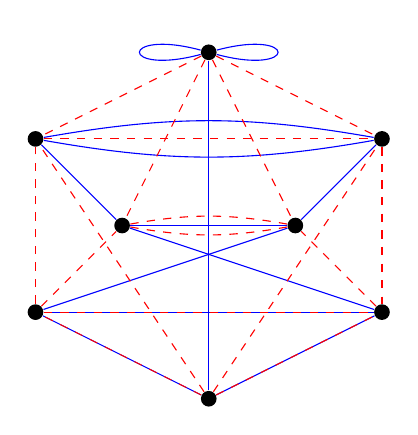
\begin{tikzpicture}[x=1.1cm,y=1.1cm]
        \begin{scope}[every node/.style={fill,black,circle,inner sep=2pt}]
          \node at (0,0)  (1){};
          \node at (0,4) (20){};
          \node at (2,1)  (16z){};
          \node at (-2,1)  (81z){};
          \node at (-1,2) (77z){};
          \node at (1,2)  (20z){};
          \node at (-2,3)  (85z){};
          \node at (2,3)  (12z){};
        \end{scope}
        
        \begin{scope}[blue,every loop/.style={looseness=50}]
          \path (1) edge (20) edge (16z) edge (81z);
          \path (20) edge[loop left] (20) edge[loop right] (20);
          \path (16z) edge (81z) edge (77z);
          \path (81z) edge (20z);
          \path (77z) edge (20z) edge (85z);
          \path (20z) edge (12z);
          \path (12z) edge[bend right=10] (85z) edge[bend left=10] (85z);
        \end{scope}
        
        \begin{scope}[red,dashed]
          \path (1) edge (85z) edge (81z) edge (12z) edge (16z);
          \path (20) edge (85z) edge (77z) edge (20z) edge (12z);
          \path (81z) edge (85z) edge (77z) edge (16z);
          \path (85z) edge (12z);
          \path (12z) edge (16z);
          \path (16z) edge (20z);
          \path (20z) edge[bend right=10] (77z) edge[bend left=10] (77z);
        \end{scope}
      \end{tikzpicture}
      \caption{The supersingular isogeny graphs of degree 2
        (blue, continuous) and 3 (red, dashed) on $\F_{97^2}$.}
      \label{fig:sidh}
    \end{minipage}
    \hfill
    \begin{minipage}{0.47\textwidth}
      \centering
      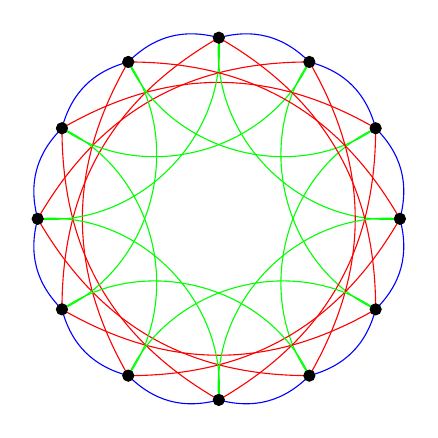
\begin{tikzpicture}
        \def\crater{12}
        \def\jumpa{-8}
        \def\jumpb{9}
        \def\diam{2.3cm}

        \foreach \i in {1,...,\crater} {
          \draw[blue] (360/\crater*\i : \diam) to[bend right] (360/\crater*\i+360/\crater : \diam);
          \draw[red] (360/\crater*\i : \diam) to[bend right] (360/\crater*\i+\jumpa*360/\crater : \diam);
          \draw[green] (360/\crater*\i : \diam) to[bend right=50] (360/\crater*\i+\jumpb*360/\crater : \diam);
        }
        \foreach \i in {1,...,\crater} {
          \pgfmathparse{int(mod(2^\i,13))}
          \let\exp\pgfmathresult
          \draw[fill] (360/\crater*\i: \diam) circle (2pt);
        }
      \end{tikzpicture}
      \caption{The supersingular isogeny graphs of degree 3 (blue), 5
        (red) and 7 (green), restricted to $\F_{89}$-rational
        isomorphism classes.\\
        Also the connected component of $j=77$ in the ordinary isogeny
        graph of $\F_{233}$ (same isogeny degrees).}
      \label{fig:csidh}
    \end{minipage}
  \end{figure}

  This graph also occurs as a connected component of infinitely many
  \emph{ordinary} graphs, for example the component containing the
  $j$-invariants $20$, $28$, $40$, $77$, $86$, $87$, $118$, $136$,
  $138$, $142$, $184$ and $194$ over $\F_{233}$ ---in the ordinary
  case, the quadratic twists form a distinct, graph-isomorphic
  component---. The edges represent $\F_{233}$-rational isogenies of
  the same degrees as before.

  This graph, is in fact none else than the Cayley graph of the
  additive group $\Z/12\Z$, generated by $1$, $3$ and $4$. The reason
  why it is such a common isogeny graph will become clear in the next
  section.

  The graph on the left is different. Its vertices are all
  supersingular $j$-invariants in the algebraic closure of
  $\F_{97}$. A classical theorem shows that all supersingular
  invariants in characteristic $p$ are defined in $\F_{p^2}$, and thus
  there is a finite number of supersingular isomorphism classes. The
  same theorem also shows that all supersingular isogenies are defined
  over $\F_{p^2}$. Figure~\ref{fig:sidh} presents two graphs (in different
  colors): a $3$-regular graph whose edges are all isogenies of degree
  $2$, and a $4$-regular one whose edges are all isogenies of degree
  $3$. The central symmetry visible to the naked eye is due to the
  Frobenius involution of $\F_{p^2}/\F_p$.

  These graphs are essentially unique: they do not occur as isogeny
  graphs of any other elliptic curves on any other field. They are
  usually called \emph{full supersingular isogeny graphs}, although
  the ``full'' and the ``isogeny'' are often dropped. The reader will find an
  interesting empirical study in~\cite{cryptoeprint:2019:1056}, and a
  database of the smallest ones in~\cite{ssingular-db}.

  
  \section{Endomorphism rings}

  Everything about isogeny graphs can be understood via
  \emph{endomorphism rings}. Endomorphisms of elliptic curves form a
  ring, under addition and composition.\footnote{A common source of
    confusion is that an extra \emph{null endomorphism} must be added
    to the set in order to make it a ring, although, by definition, a
    constant map does not qualify as an isogeny.} Their structure is
  well understood: they are free $\Z$-modules of dimension $1$, $2$ or
  $4$. There is more: if we exclude the subring $\Z\subset\End(E)$,
  any endomorphism is a quadratic integer, i.e., it is annihilated by
  a monic quadratic polynomial with integer coefficients. These
  constraints leave only a handful of possible choices.

  \begin{theorem}
    Let $E$ be an elliptic curve over a field of characteristic $p$,
    its endomorphism ring is isomorphic to one of the following:
    \begin{enumerate}
    \item the ring of integers, only if $p=0$,
    \item an order in a quadratic imaginary number field,
    \item only if $p\ne 0$, a maximal order in the quaternion algebra
      ramified at $p$ and infinity.\footnote{The reader unacquainted
        with number fields may learn about them in any book on
        algebraic number theory,
        such as~\cite{langANT,neukirch2013algebraic,Cohen1993}.  For
        quaternion algebras I recommend~\cite{Vigneras_1980,voight}.}
    \end{enumerate}
    In positive characteristic, the second case is called
    \emph{ordinary} and the third \emph{supersingular}.
  \end{theorem}

  If $\phi:E\to E'$ is an isogeny, $\hat\phi:E'\to E$ its dual, and
  $\omega:E\to E$ an endomorphism of $E$, then $\phi\circ\omega\circ\hat\phi$ is
  an endomorphism of $E'$. It stands to reason that the endomorphism
  rings of $E$ and $E'$ must be somehow related.  Indeed, to any
  separable isogeny $\phi$ we can associate its \emph{kernel ideal}
  $I_\phi\subset\End(E)$, defined by
  \[I_\phi = \bigl\{ \omega \in \End(E) \;\big\vert\; \omega(\ker\phi)
    = \{0\} \bigr\},\] %
  and it turns out we can extend\footnote{The correspondence for
    inseparable isogenies is slightly more technical, and we are
    forced to omit the details.} this correspondence to a bijection
  between isogenies and ideals.

  Then, for any ideal $I_\phi\subset\End(E)$ with associated isogeny
  $\phi:E\to E'$, we define the operation $\star$ by
  $I_\phi\star E := E'$. We say that two ideals $I,J$ are
  \emph{equivalent} if $I\star E=J\star E$, or equivalently if
  $nI=J\cdot(\omega)$ for some non-zero integer $n$ and some non-trivial principal ideal
  $(\omega)$. We call \emph{ideal class} a set of equivalent
  ideals. In general these classes do not have a simple algebraic
  structure, however, if we restrict them in an appropriate manner,
  $\star$ becomes a \emph{group action} by an \emph{ideal class
    group}. The simplest such case is the object of the
  \emph{fundamental theorem of complex multiplication}.

  \begin{theorem}[Complex multiplication]
    \label{th:cm}
    Let $\F_q$ be a finite field, let $\O\subset\Q(\sqrt{-D})$ be a
    quadratic imaginary order, denote by $\Ell_q(\O)$ the set of
    elliptic curves over $\F_q$ with endomorphism ring isomorphic to
    $\O$ and assume it is non-empty. The operation $\star$ defines an
    action of the group of invertible fractional ideals of $\O$ on
    $\Ell_q(\O)$, and the action factors through the subgroup of
    principal ideals. Said otherwise, the \emph{class group} $\Cl(\O)$
    acts regularly on $\Ell_q(\O)$.
  \end{theorem}

  Similar statements hold when $E$ is supersingular and
  $\O\subset\End(E)$ is a quadratic order. An easy case is when $E$ is
  defined over a prime field $\F_p$: then the subring
  $\End_{\F_p}(E)\subset\End(E)$ of $\F_p$-rational endomorphisms is
  isomorphic to one of $\O=\Z[\sqrt{-p}]$ or $\O=\Z[(1+\sqrt{-p})/2]$,
  and if we define $\Ell_p(\O)$ as the set of all supersingular curves
  over $\F_p$ such that $\End_{\F_p}(E)\simeq\O$, the group $\Cl(\O)$
  acts regularly on $\Ell_p(\O)$ like in the complex multiplication
  case~\cite{Delfs2016}.

  These facts explain why the graph in Figure~\ref{fig:csidh} is
  isomorphic to a Cayley graph of $\Z/12\Z$. To construct the
  examples, we chose $\O\simeq\Z[\sqrt{-89}]$, which has class group
  isomorphic to $\Z/12\Z$ and is generated by an ideal of norm $3$
  (more formally, an ideal class representing $3$), corresponding to
  isogenies of degree $3$ (the blue edges). Thus $\Ell_{89}(\O)$ is
  the set of all $\F_{89}$-rational supersingular curves, but also,
  for any $p$ such that $-89$ is a square modulo $p$, there exists a
  power $q$ of $p$ such that $\Ell_q(\O)$ is non-empty. In any of
  these cases, $\Cl(\O)$ acts faithfully and transitively on
  $\Ell_q(\O)$, and the action of a basis of elements of $\Cl(\O)$ can
  be visualized as a Cayley graph.

  While Theorem~\ref{th:cm} describes almost completely isogeny graphs
  of ordinary curves, the picture for supersingular graphs is more
  involved. Mestre~\cite{mestre86}, then Kohel~\cite{kohel} showed
  that full supersingular graphs are regular and connected, by
  relating their adjacency matrices to \emph{Hecke operators} (see
  also~\cite{emerton2002supersingular}).  Independently,
  Pizer~\cite{pizer1,pizer2}, showed that such graphs satisfy the
  \emph{Ramanujan property}, i.e., they are asymptotically optimal
  expanders~\cite{hoory2006expander}.

  
  \section{CSIDH\dots}
  And we are back to isogeny based cryptography 101: key exchange.

  Couveignes~\cite{cryptoeprint:2006:291} was the first to propose a
  key exchange scheme based on the group action of complex
  multiplication, however his work stayed mostly unknown. His ideas
  were independently rediscovered ten years later by Rostovtsev and
  Stolbunov~\cite{rostovtsev+stolbunov06}, who were the first to
  suggest isogenies may be good candidates for constructing
  quantum-resistant schemes.

  Replicating the Diffie--Hellman key exchange with a
  \emph{cryptographic group action} is almost immediate. Given a
  finite abelian group $G$ acting regularly on a set $X$, given a
  \emph{starting element} $x_0\in X$, let secret keys be random
  elements $a,b\in G$, and define public keys as $x_a = a\star x_0$
  and $x_b = b\star x_0$. Then, the shared secret is obtained as
  \[a\star x_b = (ab)\star x_0 = b\star x_a.\] %
  This key exchange is secure if the analogue of the Diffie--Hellman
  assumption holds for the group action $(G,X,\star)$.

  However, the case of the complex multiplication group action
  $(\Cl(\O), \Ell_q(\O), \star)$ is more complicated for a number of
  reasons:
  \begin{enumerate}
  \item It is usually not possible to test equality in $\Cl(\O)$, nor
    to sample uniformly from it;
  \item Evaluating $a\star x$ cannot be done in polynomial time for a
    majority of inputs $a$, even though every element $a\in\Cl(\O)$
    does have a representation that supports fast evaluation of the
    group action.
  \end{enumerate}
  These two limitations follow from two fundamental algorithmic
  obstacles:
  \begin{enumerate}
  \item The order, and thus also the group structure of $\Cl(\O)$ is
    generally unknown. Indeed, the best classical algorithm to compute
    the group structure of $\Cl(\O)$ is a type of index calculus, with
    subexponential complexity $L_{\#\O}(1/2)$. The current record is
    the computation for the class group of discriminant
    $4\cdot 587\cdot\prod_{i=1}^{73} \ell_i$, where $\ell_i$ are the
    first $73$ odd primes~\cite{AC:BeuKleVer19}, which
    took about 52 core years on an inhomogeneous
    cluster. Unfortunately discriminants used in isogeny based
    cryptography may be larger. The good news is that computing the
    structure of $\Cl(\O)$ is precisely as difficult as breaking RSA
    for a quantum computer, thus we only have to wait!
  \item The cost of evaluating the action of an ideal
    $I_\phi\subset\End(E)$ is polynomial in the norm of the ideal,
    i.e., in the degree of the associated isogeny $\phi$. This
    severely limits the kind of ideals for which it is feasible to
    evaluate the action $\star$.
  \end{enumerate}

  Before giving the solution to this conundrum, let's take a step back
  and see how classical discrete logarithms are related to Cayley
  graphs. Given a group $G$ of prime order $p$, exponentiation defines
  a regular action of $(\Z/p\Z)^\times$ on $G\setminus\{1\}$ by
  \[a\star g := g^a.\] %
  From a subset $S\subset(\Z/p\Z)^\times$, we may construct the Cayley
  graph $[(\Z/p\Z)^\times,S]$. For example, the graph in
  Figure~\ref{fig:csidh} can be equally seen as the Cayley graph of
  $(\Z/13\Z)^\times$ generated by $S=\{2,8,3\}$. The same graph can be
  equally interpreted as the graph whose vertices are non-identity
  elements of $G$, and where two vertices $g,h$ are connected whenever
  $h=g^a$ for some $a\in S$. This graph is sometimes called the
  \emph{Schreier graph} $(\star,S)$.

  Given two elements $g,h\in G$, finding a path between them in the
  Schreier graph is equivalent to computing their discrete
  logarithm. There is only one gotcha: the path must be \emph{short},
  e.g., of polynomial length in $\log(\#G)$, otherwise the solution is
  practically useless. Intuitively, the larger $S$, the smaller the
  diameter of the graph, and indeed it is well known that Cayley
  graphs tend to make good expanders.

  If we take $S$ large enough, then we even have an effective way to
  sample random elements in $G$ nearly uniformly: it is sufficient to
  start from an arbitrary generator of $G$, and perform a random walk
  of polynomial length in $\log(\#G)$. This fact can be used to
  construct a key exchange similar to Diffie--Hellman: fix a starting
  generator $g$, sample random walks
  $(a_1,\ldots,a_n), (b_1,\ldots,b_n)\in S^*$, define as public keys
  \[g^a = g^{\prod a_i}, \quad g^b = g^{\prod b_i},\] then the shared
  secret $g^{ab}$ is obtained by replaying the same random walks from
  $g^b$ and $g^a$ respectively.

  Coming back to the complex multiplication group action, Jao \emph{et
    al.}~\cite{jao+miller+venkatesan09} proved, assuming the
  generalized Riemann hypothesis, that Cayley graphs $[\Cl(\O),S]$
  form an expander family as soon as
  $\#S\in O\bigl(\log(\#\Cl(\O))^2\bigr)$. Following the previous
  sketch, we immediately obtain a key exchange scheme based on complex
  multiplication.

  \begin{description}
  \item[Setup.] Choose a quadratic imaginary order $\O$ and an
    elliptic curve $E_0 \in \Ell(\O)$. Fix a set
    $\{s_1,\dots,s_n\}\subset\Cl(\O)$ of ideal representatives of
    small norm.
  \item[Public key generation.] Sample a random integer vector
    $(e_1,\ldots,e_n)$ and construct the ideal
    \[I = \prod_{i=1}^n s_i^{e_i};\]
    output the public key $I\star E_0$.
  \item[Shared secret computation.] Given a public key $E$, and a
    secret ideal $I\subset\O$, output the shared secret $I\star E$.
  \end{description}

  This is precisely the key exchange scheme of Couveignes, Rostovtsev
  and Stolbunov, although we have left some details unspecified: how
  to choose $\O$, how to find $E_0$, how to compute the group action,
  \dots For a long time, the only known way to instantiate the scheme
  produced a system too slow to be useful in practice, a fact reported
  as recently as 2018~\cite{AC:DeFKieSmi18}. A breakthrough came the
  same year, though, with the invention of CSIDH\footnote{Acronym for
    ``Commutative Supersingular Isogeny Diffie--Hellman'', pronounced
    like \emph{``sea side''}.}~\cite{AC:CLMPR18}, an
  instantiation based on the action of $\Cl(-p)$ on the set of
  supersingular curves defined over $\F_p$. Parameters in CSIDH are
  chosen as follows:
  \begin{itemize}
  \item $p$ is a prime such that $p+1=4\prod \ell_i$, where $\ell_i$
    is a set of small odd primes. For a target classical security of
    $\lambda$ bits, $\log_2(p)$ needs to be approximately $4\lambda$.
  \item The quadratic order is $\O=\Z[\sqrt{-p}]$.  The set of ideal
    representatives of small norm is taken to be
    $s_i=(\ell_i,1-\sqrt{-p})$, for each of the $\ell_i$ in the
    factorization of $p+1$.
  \item Thanks to the constraints on $p$, the elliptic curve of
    equation $y^2=x^3+x$ is supersingular, has $\F_p$-rational
    endomorphism ring isomorphic to $\O$, and is thus taken as
    $E_0$.
  \item The secret vectors $(e_1,\ldots,e_n)$ are sampled from an integer box
    $[-B,B]^n$, such that $(2B+1)^n\approx\sqrt{p}$.
  \end{itemize}
  
  These choices make for a surprisingly simple algorithm to evaluate
  the action $\star$. Indeed, after identifying $\sqrt{-p}$ to the
  Frobenius endomorphism of any curve $E\in\Ell(\O)$, the isogeny
  kernel associated to $s_i=(\ell_i,1-\sqrt{-p})$ is simply the set
  $E[\ell_i]\cap E(\F_p)$ of $\F_p$-rational points of order
  $\ell_i$. Given this kernel, Vélu's
  formulas~\cite{velu71,moody2016analogues,PQCRYPTO:Renes18}
  efficiently compute the associated isogeny and the image curve
  $s_i\star E$ using $O(\ell_i)$ finite field operations.\footnote{In
    a recent development~\cite{bernstein2020faster}, the upper bound
    on the complexity of computing the isogeny action has been
    improved to $\tilde{O}(\sqrt{\ell_i})$.}  Furthermore, it is not
  difficult to see that the inverse ideal class $s_i^{-1}$ is
  represented by $(\ell_i,1+\sqrt{-p})$, and the associated kernel is
  the set of points of order $\ell_i$ that have abscissa in $\F_p$ and
  ordinate in $\F_{p^2}$. Thus, the action of any ideal $s_i^{\pm e}$
  can be evaluated by $e$ applications of Vélu's formulas, and the
  action of the product ideal $\prod s_i^{e_i}$ is simply the
  composition of each individual action.  The total cost of evaluating
  the CSIDH group action is thus $\sim B\sum\ell_i$ finite field
  operations, ignoring some not-so-negligible computations such as
  finding the generators of the various isogeny kernels.

  It is worth pointing out that Jao \emph{et al.}'s theorem does not
  apply to the CSIDH graph, because its degree of regularity is in
  $O(\log_2(p))$ rather than $O(\log_2(p)^2)$; nevertheless,
  reasonable heuristics let us still argue that the graph has good
  expansion properties, and thus that the distribution of public keys
  is practically indistinguishable from uniform.
  
\section{\dots and SIDH}
For all its elegance and simplicity, CSIDH has a serious drawback when
it comes to quantum security, as we shall see next. Its evil twin
SIDH\footnote{Initialism for ``Supersingular Isogeny Diffie--Hellman'',
  pronounced by spelling out the letters
  \emph{``ess-eye-dee-aitch''}.}~\cite{jao+defeo2011,defeo+jao+plut12}
was designed to overcome this limitation.

The goal of SIDH is to be able to perform a key exchange based on
random walks in the full supersingular graph. Since no group acts on
the full graph, constructing commuting isogeny walks is not obvious;
however the lack of an exploitable group action is also what makes attacking
SIDH more difficult.

But let's start from the kind of isogeny walks we perform in SIDH. As
we know, in CSIDH an isogeny walk is defined by a list
$(e_1,\dots,e_n)$ of integers. Each integer corresponds to a different
isogeny degree $\ell_i$, the magnitude $|e_i|$ indicates the number of
steps to travel along the $\ell_i$-isogeny cycle (each cycle is
represented by a different color in Figure~\ref{fig:csidh}), and the
sign of $e_i$ means ``go forward'' or ``go backward'' (the meaning to
the orientation was given by the Frobenius endomorphism).  The order
in which the different primes $\ell_i$ are processed is irrelevant, as
we know that isogenies correspond to an abelian group action.

It is absolutely necessary that CSIDH uses a fairly large collection
of primes $\ell_i$. Indeed, if the vectors $(e_1,\dots,e_n)$ are selected from a
box $[-B,B]^n$, then the number of distinct end points for these
isogeny walks is at most $(2B+1)^n$, but the cost of computing one
walk is proportional to $Bn$. Said otherwise, the only parameter in
which the key space size grows exponentially (compared to the cost of
executing the key exchange) is the number of distinct primes $\ell_i$.

Moving to the full supersingular graph the outlook changes. There are
approximately $p/12$ supersingular isomorphism classes in the
algebraic closure of $\F_p$, and they are all defined over $\F_{p^2}$.
Over $\F_{p^2}$, every supersingular curve has exactly $\ell+1$
distinct isogenies for any prime $\ell$, i.e., the $\ell$-isogeny
graph is $(\ell+1)$-regular.\footnote{A small exception must be
  granted to the curves of $j$-invariant $0$ or $1728$, which have
  out-degree $\ell+1$, but lower in-degree.} Hence, unlike in the
complex multiplication case, starting from any supersingular curve $E$
there are exactly $(\ell+1)\ell^n$ distinct
non-backtracking\footnote{Most theorems for random walks in graphs are
  stated for ordinary walks, where one undirected edge can be
  immediately followed by the same edge in the opposite
  direction. However, in our context, following an isogeny step by its
  dual is not interesting: it produces a scalar multiplication
  $[\ell]$ which is easily factored out of the walk, and does not
  contribute to the security of the cryptosystem.} $\ell$-isogeny walks
of length $n+1$, instead of just $2$. Furthermore, the Ramanujan
property proved by Pizer~\cite{pizer1,pizer2} indicates that the
induced distribution on the vertices quickly approaches the uniform
distribution as soon as $n\approx c_\ell\log(p)$ for some constant
$c_\ell$.

These facts were already exploited by Charles \emph{et
  al.}~\cite{JC:ChaLauGor09} to construct a collision resistant hash
function based on pseudo-random walks in supersingular $2$-isogeny
graphs, and their work was indeed an inspiration for SIDH.  In
principle, we would like to find a way for two parties to perform
walks in the $\ell$-isogeny graph in such a way that the walks
commute. However there is an obvious tension here: if the proverbial
Alice and Bob each perform an isogeny walk of length $n$, call them
$A$ and $B$, and if the order of $A$ and $B$ does not count, i.e.,
$A\circ B=B\circ A$, then why would the order of the steps
\emph{within} $A$ or $B$ count, in general?  Indeed we know no way to
construct commuting walks in a supersingular graph in a way that is
compatible with the security of a key exchange scheme.

The trick used by SIDH is to have Alice and Bob do walks in two
different supersingular graphs on the same vertex set (see
Figure~\ref{fig:sidh}). Fix two primes, say $2$ and $3$. Alice
performs a random walk $A$ in the $2$-isogeny graph, while Bob
performs a random walk $B$ in the $3$-isogeny graph. By coordinating
their efforts carefully, they can ensure that $A\circ B = B\circ A$,
and still get a secure key exchange protocol.

The way this works is astonishingly simple. A $2$-isogeny walk of
length $n$ is nothing else than a composition of isogenies of degree
$2$, i.e., an isogeny of degree $2^n$. Call $\phi_A$ this isogeny, and
call $R_A$ a point of order $2^n$ generating $\ker\phi_A$. Similarly,
let $\phi_B$ be a $3^m$-isogeny and let $R_B$ be a generator of its
kernel. Then $R_A+R_B$ is a point of order $2^n3^m$, and to it is
associated a unique isogeny $\phi_{AB}$ of the same degree. Then,
there exist isogenies $\phi_A'$ and $\phi_B'$ such that the following
diagram commutes
\begin{equation}
  \label{eq:sidh}
  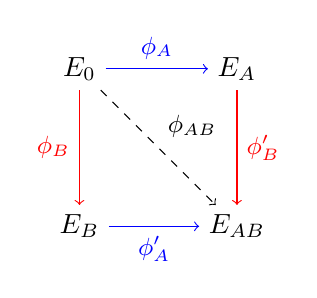
\begin{tikzpicture}[scale=2,baseline=-1cm]
    \node (E0)  at (0,0) {\(E_0\)};
    \node (EA)  at (1,0) {\(E_A\)};
    \node (EB)  at (0,-1) {\(E_B\)};
    \node (EAB) at (1,-1) {\(E_{AB}\)};
    \draw[->,font=\small]
    (E0) edge[blue] node[auto] {\(\phi_A\)} (EA)
         edge[red] node[auto,swap] {\(\phi_B\)}  (EB)
         edge[dashed] node[auto] {\(\phi_{AB}\)}  (EAB)
    (EA) edge[red] node[auto] {\(\phi_B'\)}  (EAB)
    (EB) edge[blue] node[auto,swap] {\(\phi_A'\)}  (EAB);
  \end{tikzpicture}
\end{equation}
Chasing around the diagram, it is evident that
$\ker\phi_A' = \langle\phi_B(R_A)\rangle$ and
$\ker\phi_B' = \langle\phi_A(R_B)\rangle$.

But we seem to have reached a dead end: $\phi_B$ is a secret of Bob's,
and $R_A$ is a secret of Alice; how can Bob safely make Alice aware of
the value $\phi_B(R_A)$? The trick is to define public ``torsion bases''
$E[2^n]=\langle P_A,Q_A\rangle$ and $E[3^m]=\langle P_B,Q_B\rangle$,
and to write $R_A$ (resp., $R_B$) as a secret linear combination of
$P_A,Q_A$ (resp., $P_B,Q_B$). Then, Bob transmits to Alice the values
$\phi_B(P_A),\phi_B(Q_A)$, from which Alice can compute $\phi_B(R_A)$ without
giving away her secret integers.

There is one trick left to make SIDH work. For the torsion bases and
the isogenies to have compact and efficient representations, it is
necessary to choose the curves very carefully, similarly to what we
did for CSIDH.  Ideally, we would like the torsion groups $E[2^n]$ and
$E[3^m]$ to be defined over the base field $\F_{p^2}$, so that
$P_A,Q_A,P_B,Q_B$ are represented by a pair of elements of $\F_{p^2}$
each.\footnote{One can do even better and represent $P_A,Q_A$ by a
  triplet of elements of $\F_{p^2}$~\cite{C:CosLonNae16}.} Over
$\F_{p^2}$, there are two isogeny classes of supersingular curves: one
with curves of order $(p+1)^2$, and one of order $(p-1)^2$, and their
$\ell$-isogeny graphs are isomorphic. It is customary to pick the
first and choose $p$ so that $p+1=2^n3^m$, thus fulfilling our
requirements.\footnote{Costello~\cite{AC:Costello20} has
  recently explored variants of SIDH where the two torsion groups are
  ``spread over'' the two classes of order $(p+1)^2$ and $(p-1)^2$.}

To summarize, SIDH can be instantiated as follows; we only give the
operations for Alice: for Bob, just switch the roles of $A$ and $B$.
\begin{description}
\item[Setup.] Choose a prime $p$ of the form $p+1=2^n3^m$. The starting
  curve is $E_0\;:\;y^2=x^3+x$. Select arbitrary bases
  $E[2^n]=\langle P_A,Q_A\rangle$ and $E[3^m]=\langle P_B,Q_B\rangle$.
\item[Public key generation.] Choose a random integer $r_a$, set
  $R_A=P_A+[r_a]Q_a$. Compute the isogeny $\phi_A:E_0\to E_A$ of
  kernel $\langle R_A\rangle$. Send $E_A,\phi_A(P_B),\phi_A(Q_B)$ to Bob.
\item[Shared secret computation] Upon receiving
  $E_B,\phi_B(P_A),\phi_B(Q_A)$, compute
  $R_A'=\phi_B(P_A)+[r_a]\phi_B(Q_A)$. Compute the isogeny
  $\phi_A':E_B\to E_{AB}$, output $j(E_{AB})$.
\end{description}

This particular instantiation closely matches the parameters chosen
for the NIST candidate SIKE~\cite{SIKE},\footnote{SIKE is the
  encryption scheme derived from SIDH, the difference is purely
  semantical, technical steps stay unchanged.} where the pair $(n,m)$
is one of $(216,137)$, $(250, 159)$, $(305, 192)$, $(372, 239)$,
depending on the security level.


\section{Breaking isogenies}
What does it take to break an isogeny based cryptosystem? At the base
of the pyramid, lies the fundamental problem of isogeny based
cryptography.

\begin{definition}[Isogeny walk problem]
  Let $E_0,E_1$ two elliptic curves drawn at random from some isogeny
  class over some finite field $k$, find a $k$-rational isogeny
  $\phi:E_0\to E_1$ of smooth degree.
\end{definition}

The ``smooth degree'' condition means that $\phi$ can be represented
as a walk in some $k$-rational isogeny graph, which is an effective
representation as long as the length of the walk is subexponential.
It is clear that a solution to this problem breaks CSIDH, as it
produces an ideal in the same ideal class as the secret key.  It is
less evident that it also breaks SIDH, but Galbraith \emph{et al.}
showed that this is indeed the case, assuming credible
heuristics~\cite{AC:GPST16}. Galbraith \emph{et al.}, as well as
Castryck \emph{et al.}~\cite{EC:CasPanVer20}, also showed that, for
supersingular curves, the isogeny walk problem is heuristically
equivalent to the following one.

\begin{definition}[Endomorphism ring problem]
  Given a random supersingular curve $E/\F_{p^2}$, compute a basis of
  its endomorphism ring.
\end{definition}

These two problems are the mainstays of isogeny based cryptography:
break them, and all the field evaporates. However, no cryptosystem is
actually based on them: in every case, some stronger assumption is
needed to prove their security. For CSIDH, for example, the curve
$E_0$ is usually fixed, and its endomorphism ring known. This is not a
major problem if the curve $E_1$ is uniformly random: indeed, an
algorithm solving this specialized variant of the problem can be
applied twice to solve the general instance. However, in CSIDH the
curve $E_1$ is not provably uniformly distributed, but rather assumed
to be computationally indistinguishable from random. Admittedly, this
is a minor departure from the original problem, and there is a
consensus that the security of CSIDH is not far from that of the
isogeny walk problem.

The situation of SIDH is more delicate:
\begin{itemize}
\item The curve $E_0$ is also fixed and of known endomorphism ring;
\item The curve $E_1$ is very far from being uniformly random, as it
  is at distance $\approx\log_\ell(p)/2$ from $E_0$, considerably
  shorter than the diameter of the graph;
\item On top of $E_1$, the SIDH protocol also publishes the evaluation
  points $\phi(P_B)$ and $\phi(Q_B)$, from whose knowledge one can
  compute the action of $\phi$ on any point of $E_0[3^m]$ (change $B$
  to $A$ and $3$ to $2$ for Bob's isogeny).
\end{itemize}

The \emph{SIDH assumptions} essentially state that it is fine to give
out this additional information, however they are widely believed to
be considerably stronger than the isogeny walk assumption, as
indicated by the existence of \emph{torsion point attacks} on
overstretched variants of
SIDH~\cite{AC:Petit17,EPRINT:KMPPS20,cryptoeprint:2021:282}.

Finally, some may object that the prime $p$ used in SIDH or CSIDH has
a very special form, and this should be taken into account when
evaluating the strength of the related assumptions. However, using
special primes for efficiency has been a common practice in elliptic
curve cryptography for decades, and it is widely believed that such
specialization has negligible impact on security.

It thus appears that from an assumption ``quality'' perspective CSIDH
is better positioned than SIDH.  Unfortunately the order is reversed
when we look at actual attacks.  Indeed the isogeny walk assumption is
not a single one, but rather a family of assumptions: one for each
isogeny class considered. The isogeny class of SIDH comprises all
supersingular curves over $\F_{p^2}$, and for that class no algorithm
better than exponential is known to solve the isogeny walk problem.
For the isogeny classes considered in CSIDH or in the earlier
Couveignes--Rostovtsev--Stolbunov protocols, instead, a powerful
quantum algorithm due to Kuperberg solves the problem in
subexponential
time~\cite{regev04,Kup,Kuperberg2013,childs2014constructing}.

Kuperberg's is a generic algorithm for the \emph{abelian hidden shift
  problem}, also known as the \emph{dihedral hidden subgroup problem}:
given a regular abelian group action $(G,X,\star)$ and a pair
$x_0,x_1\in X$, given quantum access to an oracle evaluating
$g\star x_0$ for arbitrary $g$, it finds the unique $\bar{g}$ such
that $x_1=\bar{g}\star x_0$. Its asymptotic complexity is roughly
$\exp\bigl(\sqrt{\log(\#G)}\bigr)$, and thus CSIDH parameters must
scale quadratically with the security level.  However, the exact
quantum security of concrete CSIDH parameters is the subject of a
heated debate, and a consensus has yet to be
reached~\cite{BIJ18,Jao-etal-kuperberg-2018,EC:BLMP19,EC:BonSch20,EC:Peikert20,cryptoeprint:2020:1520}.

On the classical front, things are simpler. The best classical attack
on CSIDH has been known for 20 years: it is a simple
meet-in-the-middle algorithm on the graph, running two pseudo-random
walks in parallel until they
meet~\cite{Gal,EC:GalHesSma02,galbraith+stolbunov11,Delfs2016}.  The
CSIDH graph contains $O(p^{1/2})$ vertices, and thus the
meet-in-the-middle attack finds a solution in $O(p^{1/4})$ steps on
average, using a negligible amount of memory if a Pollard-rho style
technique is used for collision detection. This justifies the 128-bits
of classical security claim for the 511 bits prime CSIDH-512.

The same collision finding algorithm works equally well on the full
supersingular graph; since the graph has $\approx p/12$ vertices, the
algorithm runs in $O(\sqrt{p})$ time.  In practice, Delfs and
Galbraith~\cite{Delfs2016} recommend working in two steps:
\begin{enumerate}
\item Find paths from $E_0\to E_0'$ and $E_1\to E_1'$ to curves
  $E_0',E_1'$ defined over $\F_p$;
\item Use collision finding over the CSIDH graph to connect the paths.
\end{enumerate}
While the asymptotic complexity is the same, this algorithm produces
shorter walks and is easier to parallelize; its quantum version using
Grover search runs in $O(p^{1/4})$ operations~\cite{INDOCRYPT:BiaJaoSan14}.

However neither algorithm is appropriate for SIDH. Indeed, as we
mentioned, the secret isogeny in SIDH has unusually small degree
$\approx 2^n\approx 3^m\approx \sqrt{p}$. Let's assume for
concreteness that the degree is $2^n$, then we may compute two sets:
the set $T_0$ of all curves at distance $\lceil n/2\rceil$ from $E_0$,
and $T_1$ of those at distance $\lfloor n/2\rfloor$ from $E_1$.  We
expect $T_0$ and $T_1$ to intersect in a single point, which is
sometimes called a \emph{claw} of $T_0$ and $T_1$.  Using a $O(1)$
access time structure such as a hash table to store, say, $T_0$, this
algorithm requires $O(p^{1/4})$ time and storage. Considerably better
than the generic one.

It is however unrealistic to assume constant time access to such a
huge amount of memory. Van Oorschot and Wiener's parallel collision
search~\cite{JC:VanWie99} provides a much more realistic solution to
the claw finding problem, performing well in practice on parallel
architectures with a limited amount of memory; with a constant amount
of memory, it runs in asymptotic time $O(p^{3/8})$. The application to
SIDH was analyzed in detail by Adj \emph{et al.}~\cite{SAC:ACCMR18},
then by Costello \emph{et al.}~\cite{PKC:CLNRV20}, and their
conclusions were used to set parameters for the NIST candidate SIKE.

We note that no known attack is capable of exploiting the knowledge of
the action of the secret isogeny on the torsion bases. So called
\emph{torsion point attacks}~\cite{AC:Petit17,EPRINT:KMPPS20,cryptoeprint:2021:282} seem so
far to only give an advantage against ``overstretched'' versions of
SIDH where the degrees of the isogenies are exponentially larger than
$\sqrt{p}$. It is an open question to determine whether the torsion
point information in SIDH can be exploited in an attack.

Finally, quantum attacks. A generic claw finding algorithm by
Tani~\cite{tani2009claw} is claimed to break SIDH using $O(p^{1/6})$
time and memory. However, a more in-depth analysis of the claims
reveals that Tani's algorithm has no advantage over a simpler Grover
search, and has thus a cost of $O(p^{1/4})$ at best, providing no
speed-up over classical algorithms~\cite{C:JaqSch19}. Quantum
accelerations of van Oorschot and Wiener's collision search have
recently been analyzed and shown not to invalidate the security claims
of SIKE either~\cite{EPRINT:JaqSch20}.

CSIDH and SIDH are not the only existing isogeny based schemes.  A
larger variety of assumptions exists to support post-quantum
signatures, identification protocols, oblivious transfer, and many
more. Nevertheless, the best available attacks always come down to
claw finding or Kuperberg's algorithm, depending on the target.

\section{What now?}

Let us come full circle and have a look back at Pedersen's
commitments. There, we needed $g$ and $h$, two random generators of a
group $G$, and we formed the commitment $g^mh^r$ for message $m$ and
randomness $r$.  Trying to port Pedersen's idea to isogenies, we may
be tempted to interpret $g$ and $h$ as two distinct starting points in
an isogeny graph, $m$ and $r$ as isogeny walks, $g^m$ and $h^r$ as
their endpoints, or as $m\star g$ and $r\star h$ for those who prefer
ideal action notation. However we are faced with two difficulties:
\begin{itemize}
\item What meaning to give to the product $g^m\cdot h^r$? In a group,
  this is a natural operation with homomorphic properties. But
  elliptic curve invariants of $m\star g$ and $r\star h$ do not
  support a natural homomorphic operation, and thus the hiding
  properties of Pedersen's commitment are lost.
\item Recall that the discrete logarithm $\log_g(h)$ must be unknown
  to the committer for the commitment to be binding. How does one
  ensure that? In principle there could be a trusted authority who is
  in charge of generating $g$ and $h$ honestly, so that $\log_g(h)$ is
  unknown to anyone.

  In practice, trusted authorities are a burden, but there is a much
  simpler option available for many discrete logarithm groups $G$. A
  surjective function $H:\Z\to G$ is called a \emph{hash into $G$} if
  given $(x,y,H(x),H(y))$ it is hard to compute $\log_{H(x)}(H(y))$. A
  non-example of hash is the map $x\mapsto g^x$ for some fixed
  generator $g$. An example of hash into the multiplicative group
  $\F_p^\times$ of a finite field is the map
  $x\mapsto (x\bmod(p-1)) + 1$.  A hash into $G$ can be used to
  generate Pedersen's base elements by setting $g=H(r_1)$ and
  $h=H(r_2)$ from some verifiable (pseudo)-random integers $r_1,r_2$
  (e.g., some parts of the digits of $\pi$).

  In the realm of isogenies there is no efficient \emph{hash into
    interesting isogeny classes}: we do not know how to generate
  random supersingular curves over $\F_p$, or over $\F_{p^2}$, other
  than by starting from a well known supersingular elliptic curve
  (e.g., $y^2=x^3+x$) and performing a long enough random walk in some
  isogeny graph. This generation process is clearly the isogeny graph
  equivalent of the non-hash $x\mapsto g^x$.  In fact, defining an
  efficient \emph{hash into the supersingular set} is one of the major
  open questions in isogeny based
  cryptography~\cite{galbraith2018computational}, and the most
  ``obvious'' ideas have already been ruled
  out~\cite{EC:CasPanVer20,love2020supersingular}.
\end{itemize}

There is no evidence that hashing in the supersingular set should be
hard, and solving this problem would pave the way to many
applications, such as making the SIDH assumptions weaker by using a
verifiably random starting curve $E_0$, removing trusted setups from
some protocols~\cite{AC:DMPS19,EPRINT:BurDeF20}, constructing
efficient oblivious pseudo-random functions from
CSIDH~\cite{jarecki2016highly}, and certainly many more.

The lack of a homomorphic operation on SIDH or CSIDH public keys,
though, is an even greater problem. Not only it breaks the idea behind
Pedersen commitments, but it is also the main obstacle to translating
to the isogeny setting efficient discrete logarithm signature schemes
such as Schnorr's~\cite{C:Schnorr89} or ECDSA, and many more basic
protocols known from discrete logarithms.

Which naturally brings us to the topic of signatures: as the reader
may know, no isogeny based signatures were submitted to the NIST
competition. Indeed, isogeny based signatures tend to be extremely
large and inefficient. The reason is that they are all obtained by
applying the Fiat-Shamir transform~\cite{C:FiaSha86} to hundreds of
parallel executions of an interactive identification protocol, thus an
SIDH or CSIDH based signature typically costs hundreds of times more
than the corresponding key exchange scheme.

There is not much to SIDH signatures: they consist in proving
knowledge of a secret isogeny by committing to the curves of a
commutative square like in Eq.~\eqref{eq:sidh}, and then revealing
some but not all of the involved isogenies~\cite{defeo+jao+plut12}.
In practice they make for signatures in the hundreds of kilobytes,
taking seconds to generate and verify~\cite{FC:YAJJS17}.

CSIDH signatures offer more variety. They are somehow similar to
discrete logarithm signatures: to prove knowledge of a secret ideal
$S$ such that $E_p=S\star E_0$, they commit to a random curve
$E_r=R\star E_0$, then reveal $RS^{-b}$, in response to a binary
challenge $b\in\{0,1\}$. Compare this to Schnorr signatures where
knowledge of the secret exponent in $g^s$ is proven by committing to
$g^r$ and then revealing $r-cs$ for some challenge $c\in\Z/p\Z$. With
such a large challenge space, the Schnorr protocol needs to be
executed only once in order to produce an unforgeable signature. In
contrast CSIDH can support a larger space only at the cost of an
exponential increase in public key size: this produces decently short
signatures, at the cost of several minutes for
signing~\cite{EC:DeFGal19}. Signing times can be considerably reduced,
though, if the structure of the class group is pre-computed, an
extremely expensive task that we already discussed previously. This is
the idea behind CSI-FiSh~\cite{AC:BeuKleVer19}, the only
practically usable isogeny based signature until recently.

A third family of isogeny signatures is based on different assumptions
than CSIDH or SIDH. At the hearth of these signatures, there is an
interactive protocol to prove knowledge of the endomorphism ring of a
supersingular curve; we already saw that this is heuristically
equivalent to knowing an isogeny walk between a special starting curve
such as $y^2=x^3+x$, and a random curve $E_p$. The idea is similar to
CSIDH based signatures: first commit to a random curve
$E_r=R\star E_p$, then respond to a challenge by revealing some ideal
related to the secret. The first such
protocol~\cite{AC:GalPetSil17,JC:GalPetSil20} only accepted binary
challenges and was notoriously difficult to implement, it has thus
always been viewed as a purely theoretical effort. In a recent
breakthrough, SQISign, a similar signature scheme with exponentially
large challenge space, has been introduced~\cite{AC:DKLPW20}.  SQISign
is not easy to implement, nor to analyze, however it boasts the
shortest signature and public key combined size among all post-quantum
candidates, by a fair margin. Signing time is not exactly fast, in the
order of seconds, but verification is comparable in speed to SIDH or
CSIDH.

To summarize, despite the similarities between CSIDH/SIDH and classic
Diffie--Hellman, several challenges materialize when trying to rebuild
on them most cryptographic protocols that we used to take for granted.
Highly advanced techniques are needed even for the relatively basic
task of signing, and for most other protocols we do not even have an
isogeny based solution yet. Fortunately, there is a vast space of
cryptographic possibilities as of yet unexplored.

At present, research on isogeny based cryptography mainly focuses on
three areas: efficient implementations, both in software and hardware;
cryptanalysis, both mathematical and physical; and achieving new
primitives. I am happy to remark that there is more work in each of
these areas than I could possibly cite in this short survey.

Turning to more prospective research, isogeny graphs of higher
dimensional abelian varieties are still an insufficiently researched
area. While some preliminary results indicate that they might not be
the best candidates for basic schemes such as key
exchange and hash functions~\cite{PQCRYPTO:FlyTi19,10.1515/jmc-2019-0021,PQCRYPTO:CosSmi20},
there is still hope that the additional structure may be used to
construct advanced functionalities. Another promising source of
advanced protocols comes from the interplay between isogenies and
pairings. Although it clearly cannot lead to post-quantum schemes, it
has been recently used to realize some unique \emph{time-release}
primitives~\cite{AC:DMPS19,EPRINT:BurDeF20}.

My feeling is that we are only scratching the surface of isogeny based
cryptography, and that much more is to come. I hope this short and
incomplete summary will motivate many of you to look more in depth
into these topics!

\end{otherlanguage}

\bibliographystyle{plainurl}
\bibliography{local,cryptobib/abbrev3,cryptobib/crypto,isogenies-bib/isogenies}

\EndContrib


%%% Local Variables:
%%% mode: latex
%%% TeX-master: "plain"
%%% End:

% LocalWords:  isogeny additively morphisms morphism supersingular
% LocalWords:  isogenies undirected expander quaternion endomorphism
% LocalWords:  monic Cayley discriminants inhomogeneous instantiation
% LocalWords:  homomorphic
